\section{Komponentendiagramm}

Für eine klare funktionale Übersicht auf der vorliegenden Diplomarbeit
wurde ein sogenanntes Komponentendiagramm für das technische System von Relaxoon erstellt.
Da Relaxoon eine Applikation ist, die auf Mobilgeräten läuft,
wurde für die Entwicklung das cross-plattform \textbf{J}ava\textbf{S}cript  (js)
Framework ''React Native'' eingesetzt. Damit der Kunde Inhalte in die App hinzufügen kann,
wurde ein ''Node.js'' basiertes Headless CMS
namens “Strapi” verwendet.

Für die Kommunikation zwischen Frontend und Backend wird REST verwendet.
Für die Persistierungsebene hat sich das Team für ''PostgreSQL'' entschieden.


\begin{figure}[H]
    \centering
    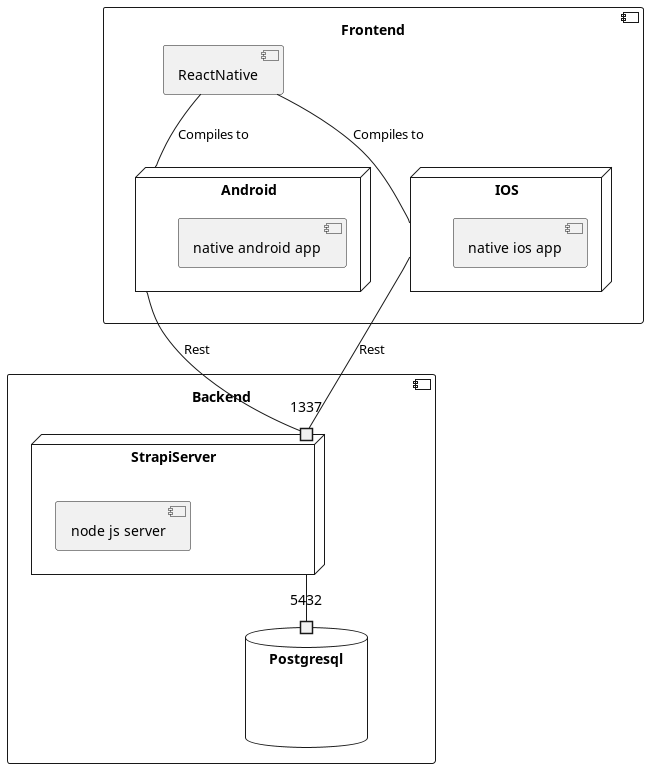
\includegraphics[width=\textwidth]{./pics/system-architektur.png}
    \caption{Systemarchitektur}
    \label{fig:Systemarchitektur}
\end{figure}